% screenshots generated with the following command, then <Alt> + <PrtSc>:
% firefox -chrome http://localhost:8080/barebones-spring-mvc/employees -width 640 -height 480
\documentclass{article}
\usepackage{graphicx}
\usepackage[
	pdftex,
	colorlinks=true,
	linkcolor=black,
	urlcolor=blue,
	bookmarks=true,
	pdfpagemode=UseOutlines,
	pdftitle={Barebones Spring MVC},
	pdfauthor={James Douglas},
	pdfkeywords=,
	pdfsubject=,
	pdfcreator=Vim,
	pdfproducer=LaTeX
	]{hyperref}
\usepackage{listings}
\usepackage{fullpage}
\usepackage{color}
\usepackage{textcomp}
\usepackage{float}
\setlength{\parindent}{0pt}
\setlength\fboxsep{0pt}
\setlength\fboxrule{0.5pt}
\lstset{
	frame=single,
	backgroundcolor=\color[rgb]{0.96,0.96,0.96},
	tabsize=4,
	language=java,
        basicstyle=\footnotesize,
        upquote=true,
        aboveskip={1.5\baselineskip},
        columns=fixed,
        showstringspaces=false,
        extendedchars=true,
        breaklines=false,
        identifierstyle=\ttfamily,
        keywordstyle=\color[rgb]{0,0,1},
        commentstyle=\color[rgb]{0.133,0.545,0.133},
        stringstyle=\color[rgb]{0.627,0.126,0.941},
	xleftmargin=15pt
}
\begin{document}
\title{Barebones Spring MVC}
\author{James Douglas\\\href{http://www.earldouglas.com/}{www.earldouglas.com}}
\maketitle
\tableofcontents
\newpage
\setlength{\parskip}{\baselineskip}
\pagebreak
\section{About This Book}

This is a book about Java Web application development using the Spring MVC framework.  It distills much of what I have learned from developing enterprise applications with Spring MVC, guiding usage of the components of Spring MVC that I most frequently encounter in practice and on discussion forums.  This book provides a brief overview of these components by taking you through the development of an example Spring MVC application from scratch.

My goals in writing this book are to guide developers who are unfamiliar with Spring MVC, and to supply a convenient reference to more seasoned developers.

\subsection{Intended Audience}

This book is written for developers who are interested in working with Spring MVC, whether they are newcomers or have been working with it for years.  It assumes basic familiarity with Spring and Java Web applications, though I have included links to reference information to help fill these gaps.

I generally don't build a Spring MVC application from scratch, opting instead to build upon a framework I have already prepared, or a sample I have already developed.  Since understanding the fundamental concepts is in no way the same as generating boilerplate code from memory, I find it valuable to maintain a barebones framework from which to springboard new project development.

\subsection{Topics Covered}

The following components of Spring MVC are covered:

\begin{itemize}
\item Core Spring MVC
\item Server-side validation
\item Rich client-side validation
\item Security
\item Database integration
\item RESTful Web services
\item Externalization and Internationalization
\end{itemize}

This book does not cover advanced, uncommon, or deep-dive topics into Spring MVC, Spring Web Flow, Spring JavaScript, JavaScript frameworks, etc., although there is some basic usage of both Spring JavaScript and the Dojo Toolkit's UI library Dijit.  Instead, this book focuses on the development of an example application which features the common Spring MVC components.

\pagebreak
\section{Example Application}

This book is based on a minimal example application which serves two goals: to provide a useful foundation in something not unlike a real-world application, and to avoid diving into a specific problem domain which eclipses the concepts as they are presented.

The example application is a limited employee directory. A user interacts with a Web front-end to view a list of employees, add new employees, and edit or delete existing employees.

\vspace{10pt}
\begin{figure}[H]
\begin{center}
\fbox{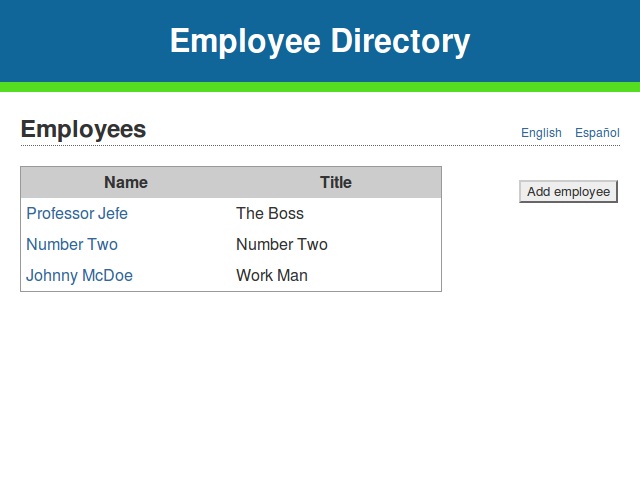
\includegraphics[width=3.2in,height=2.4in]{images/core/view-employees.png}}
\end{center}
\caption{The \emph{employees} view}
\label{fig:core/view-employees}
\end{figure}

Figure \ref{fig:core/view-employees} shows the main view of the Employee Directory.  It lists all employees in the directory, provides links to view and edit the details of each, and includes a button for adding a new employee to the directory.

\vspace{10pt}
\begin{figure}[H]
\begin{center}
\fbox{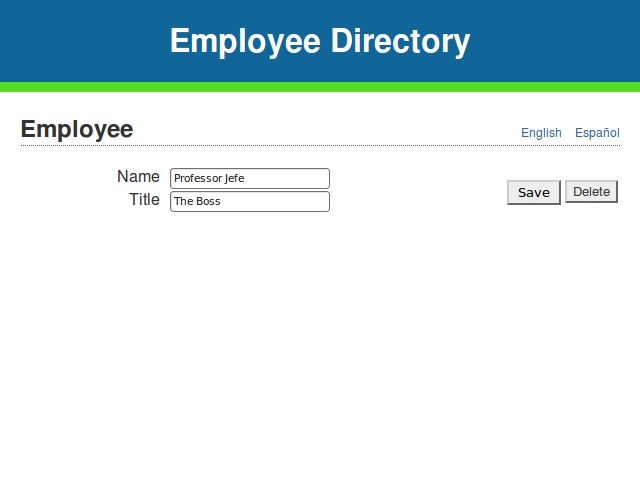
\includegraphics[width=3.2in,height=2.4in]{images/core/view-employee.png}}
\end{center}
\caption{The \emph{employee} view}
\label{fig:core/view-employee}
\end{figure}

Figure \ref{fig:core/view-employee} shows a detailed view of a single employee.  When the details of an employee are viewed, or when a new employee is to be added, this view is presented.

\subsection{Application Skeleton}

The Employee Directory is structured as a Maven project.  At the root of the project is the POM, where dependencies and other project configuration is maintained. Application source code is placed in \texttt{src/main/java}, with corresponding configuration in \texttt{src/main/resources}.  Web application content and configuration is within \texttt{src/main/webapp}.  This includes the \texttt{web.xml} deployment descriptor, the JSP view templates, and other Web content (stylesheets, images, etc.).

\subsection{Source Code}

This book includes snippets of source code for the Employee Directory.  The full source code is available online, from \href{http://www.earldouglas.com/barebones-spring-mvc}{http://www.earldouglas.com/barebones-spring-mvc}.  I recommend keeping it handy for reference and experimentation as you progress through the content.

Source code included in this book is formatted as follows.

\lstinputlisting[caption=CodeConventions.java]{source-code/CodeConventions.java}

\subsection{Section References}

\begin{itemize}
\item The Maven POM is covered in detail in the \href{http://maven.apache.org/pom.html}{Apache Maven Project Reference}.
\item The \texttt{web.xml} deployment descriptor, and the WAR file format in general, are covered in \href{http://en.wikipedia.org/wiki/WAR_(Sun_file_format)}{Wikipedia}.
\end{itemize}

\pagebreak
\section{Core Application}

\subsection{Components}

The core of the Employee Directory is the largest single segment of its construction.  It consists of an in-memory repository of employees, with an HTML front-end for user interaction, using the following components:

\subsubsection{Classes}
\begin{itemize}
\item \texttt{Employee}: a domain class representing an employee
\item \texttt{EmployeeService}: a simple CRUD-like interface for fetching, saving, and deleting Employees
\item \texttt{InMemoryEmployeeService}: an EmployeeService implementation which contains an in-memory collection of Employees
\item \texttt{BindableEmployee}: a flat class designed to bind to HTML forms
\item \texttt{EmployeeController}: a Spring MVC controller to interact with the user
\end{itemize}

\subsubsection{Views}
\begin{itemize}
\item \texttt{employee.jsp}: a template for an HTML form for creating or updating an employee
\item \texttt{employees.jsp}: a template for a list of employees in the Employee Directory
\end{itemize}

\subsubsection{Configuration}
\begin{itemize}
\item \texttt{style.css}: template CSS configuration for the views
\item \texttt{pom.xml}: project dependencies and management
\item \texttt{web.xml}: the J2EE Web deployment descriptor containing the Spring DispatcherServlet, the Front Controller for a Spring MVC application
\item \texttt{spring-mvc-servlet.xml}: the Spring configuration for the various Spring beans and Spring infrastructure
\end{itemize}

\subsection{Classes}

At the architectural bottom of the code is the domain class \texttt{Employee}.

\vspace{10pt}
\begin{figure}[H]
\begin{center}
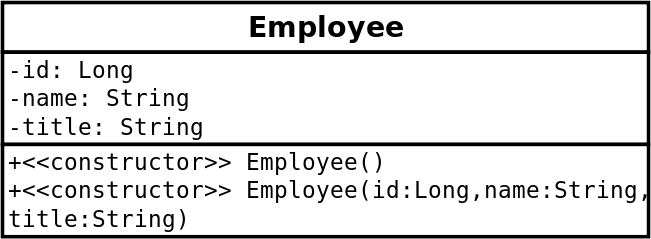
\includegraphics[scale=0.5]{images/core/class-Employee.png}
\end{center}
\caption{The \texttt{Employee} class}
\label{fig:core/Employee}
\end{figure}

\lstinputlisting[caption=Employee.java]{source-code/core/Employee.java}

A service interface is defined by \texttt{EmployeeService}, which provides the standard CRUD behavior.

\vspace{10pt}
\begin{figure}[H]
\begin{center}
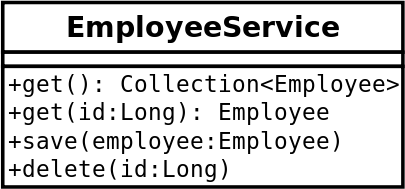
\includegraphics[scale=0.5]{images/core/class-EmployeeService.png}
\end{center}
\caption{The \texttt{EmployeeService} interface}
\label{fig:core/EmployeeService}
\end{figure}

\lstinputlisting[caption=EmployeeService.java]{source-code/core/EmployeeService.java}

A simple in-memory \texttt{EmployeeService} is implemented by \texttt{InMemoryEmployeeService}.

\vspace{10pt}
\begin{figure}[H]
\begin{center}
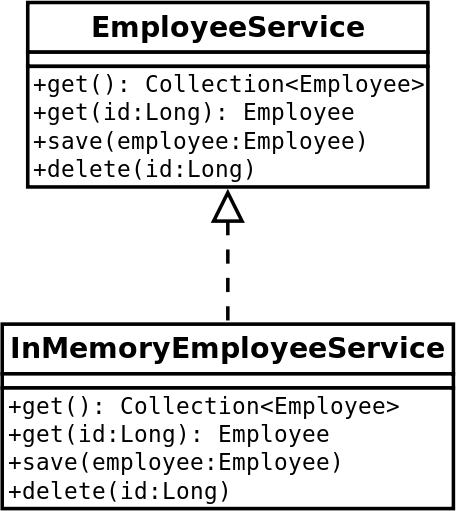
\includegraphics[scale=0.5]{images/core/class-EmployeeService-InMemoryEmployeeService.png}
\end{center}
\caption{The \texttt{EmployeeService} interface and \texttt{InMemoryEmployeeService} class}
\label{fig:core/EmployeeService-InMemoryEmployeeService}
\end{figure}

\lstinputlisting[caption=InMemoryEmployeeService.java]{source-code/core/InMemoryEmployeeService.java}

This service implementation will provide core services to the Web front-end, implemented as \texttt{EmployeeController}.  The \texttt{EmployeeController} is responsible for handling HTTP requests, and translating between the UI model and the domain model classes.

\vspace{10pt}
\begin{figure}[H]
\begin{center}
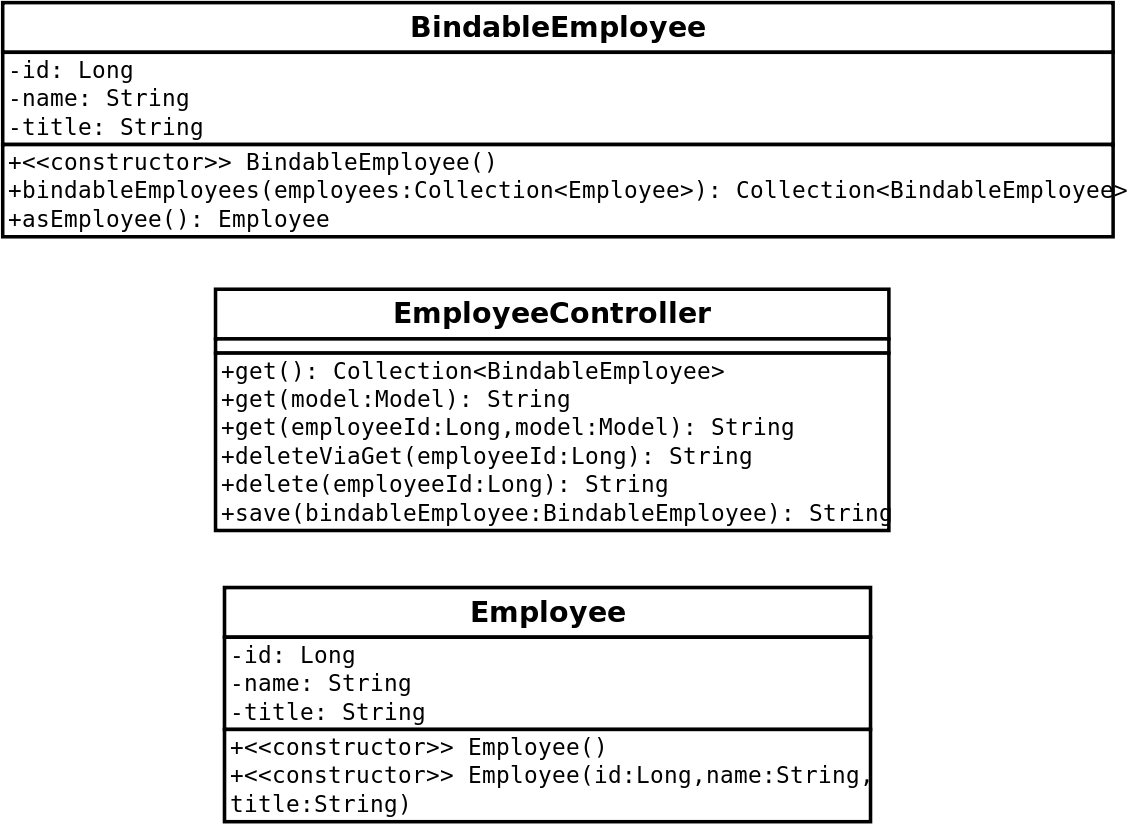
\includegraphics[scale=0.5]{images/core/class-EmployeeController-BindableEmployee-Employee.png}
\end{center}
\caption{The \texttt{BindableEmployee}, \texttt{EmployeeController}, and \texttt{Employee} classes}
\label{fig:core/EmployeeController-BindableEmployee-Employee}
\end{figure}

\lstinputlisting[caption=EmployeeController.java]{source-code/core/EmployeeController.java}

There are several things going on in \texttt{EmployeeController}.  The class is annotated with \texttt{@Controller} to indicate to Spring its function as an MVC controller and its candidacy for component scanning by the Spring container.  In addition, it is annotated with a class-level \texttt{@RequestMapping} to base all of its method-level \texttt{@RequestMapping}s on a top-level URL pattern.  Each method is also annotated with \texttt{@RequestMapping} to further constrain their specific associated request patterns.

The \texttt{get(Long, Model)}, \texttt{deleteViaGet(Long)}, and \texttt{delete(Long)} methods are each configured to map to RESTful URLs which contain the identifier of the \texttt{Employee} object on which to operate.

The \texttt{save(BindableEmployee} method contains no URL information in its \texttt{@RequestMapping}, so it will map simply to \texttt{/employees}, that of the class-level annotation.  This is in contrast to the other methods, such as \texttt{get(Model)}, which specifies \texttt{/new}.  This combines with the class-level annotation to map to \texttt{/employees/new}.

All of the methods specify a HTTP request method in the RESTful style.

\texttt{EmployeeController} presents \texttt{Employee}-like data to the user both as textual data and as an HTML form.  This is cause for a special class to be designed with the Web UI in mind, specifically to bind to the HTML form.  This role is filled by \texttt{BindableEmployee}.

\lstinputlisting[caption=BindableEmployee.java]{source-code/core/BindableEmployee.java}

\texttt{BindableEmployee} knows both how to convert itself into the domain class \texttt{Employee} via its \texttt{asEmployee()} method and how to convert a collection of instances of \texttt{Employee} into a collection of instances of \texttt{BindableEmployee}.  This is a convenient location for this functionality, and an important one as well.  Because this conversion is only concerned with connecting the domain to a thin Web layer, the appropriate location for related computation is in the Web layer and out of the domain.

That's all the Java code there is to write.  Simple!

\subsection{View Templates}

Next, the view templates are defined.

\texttt{employee.jsp} uses Spring's \texttt{form} tag library to build a form with text inputs for the name and title of an employee.

\vspace{10pt}
\begin{figure}[H]
\begin{center}
\fbox{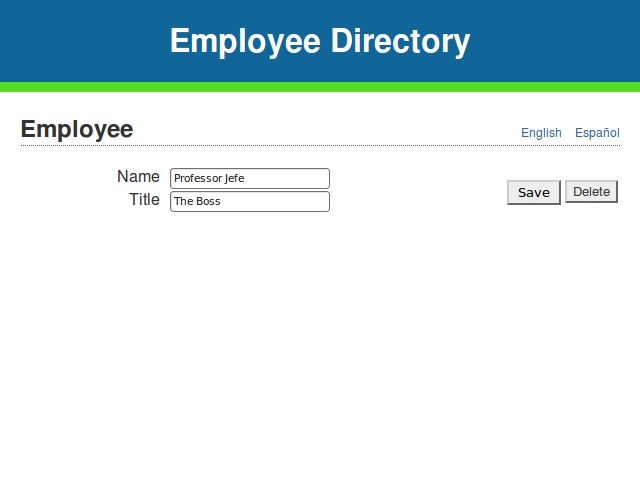
\includegraphics[width=3.2in,height=2.4in]{images/core/view-employee.png}}
\end{center}
\caption{The \texttt{employee} view}
\label{fig:core/view-employee-1}
\end{figure}

\lstinputlisting[caption=employee.jsp]{source-code/core/employee.jsp}

\texttt{employees.jsp} displays a list of the employees in the system, provides links to edit each, and includes a button to add a new employee to the system.

\vspace{10pt}
\begin{figure}[H]
\begin{center}
\fbox{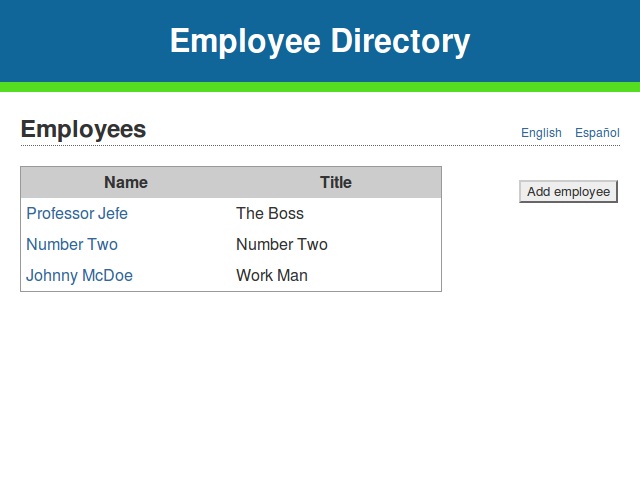
\includegraphics[width=3.2in,height=2.4in]{images/core/view-employees.png}}
\end{center}
\caption{The \emph{employees} view}
\label{fig:core/view-employees-1}
\end{figure}

\lstinputlisting[caption=employees.jsp]{source-code/core/employees.jsp}

\subsection{Spring Configuration}

Next, the Spring configuration is defined.

\lstinputlisting[caption=spring-mvc-servlet.xml,language=xml]{source-code/core/spring-mvc-servlet.xml}

The \texttt{<mvc:annotation-driven />} element tells Spring to create a \texttt{DefaultAnnotationHandlerMapping} bean to set up handling of the \texttt{@RequestMapping} annotations in \texttt{EmployeeController}, while the lone bean definition registers a view resolver which looks for JSPs by view name.  The \texttt{EmployeeController} is picked up by the \texttt{component-scan}, instantiated, and mapped to its applicable requests by \texttt{DefaultAnnotationHandlerMapping}.

Next, we have our Web deployment descriptor.

\lstinputlisting[caption=web.xml,language=xml]{source-code/core/web.xml}

Note that since the \texttt{DispatcherServlet} is named \texttt{spring-mvc}, by convention the Spring configuration is retrieved from \texttt{/WEB-INF/spring-mvc-servlet.xml}.

\subsection{Section References}

\begin{itemize}

\item The \texttt{component-scan} tag, the \texttt{@Controller} annotation, and classpath scanning is covered in the \href{http://static.springsource.org/spring/docs/3.0.x/spring-framework-reference/html/beans.html#beans-classpath-scanning}{Spring 3 Reference, section 3.10}.

\item The \texttt{@RequestMapping} annotation is covered in the \href{http://static.springsource.org/spring/docs/3.0.x/spring-framework-reference/html/mvc.html#mvc-ann-requestmapping}{Spring 3 Reference, section 15.3.2}.

\item The Spring form tag library is covered in the \href{http://static.springsource.org/spring/docs/3.0.x/spring-framework-reference/html/view.html#view-jsp-formtaglib}{Spring 3 Reference, section 16.2.4}.

\item The \texttt{DefaultAnnotationHandlerMapping} and handler mappings in general are covered in the \href{http://static.springsource.org/spring/docs/3.0.x/spring-framework-reference/html/portlet.html#portlet-handlermapping}{Spring 3 Reference, section 18.5}.

\item Of note is Spring's convention over configuration support with the \texttt{ControllerClassNameHandlerMapping} class, covered in the \href{http://static.springsource.org/spring/docs/3.0.x/spring-framework-reference/html/mvc.html#mvc-coc}{Spring 3 Reference, section 15.10}.

\item Spring's comprehensive REST support is covered in the \href{http://static.springsource.org/spring/docs/3.0.x/spring-framework-reference/html/new-in-3.html#d0e1188}{Spring 3 Reference, section 2.5.6.1}.

\end{itemize}

\pagebreak
\section{Server-Side Validation}

Form validation goes hand-in-hand with Web applications, and server-side form validation is an easy addition to the core application.  JSR-303 Bean Validation specifies annotations for declarative validation rules, which can be standardized across the layers of an enterprise application from the database to the user interface.

\subsection{Additions}

The following additions are required:

\begin{itemize}
\item The JSR-303 validation API \texttt{javax.validation} to the Maven POM
\item The \texttt{@Valid} annotation to controller method inputs
\item \texttt{Errors} objects to controller method inputs for view error binding
\item JSR-303 annotations to \texttt{BindableEmployee.java}
\item A JSR-303-backed \texttt{Validator} to the Spring context
\item A JSR-303 reference implementation \texttt{hibernate-validator} to the Maven POM
\item \texttt{<form:errors />} elements to \texttt{employee.jsp}
\end{itemize}

\subsection{Classes}

There is only one controller method with input: \texttt{save(BindableEmployee)}.  The \texttt{BindableEmployee} parameter is annotated with \texttt{@Valid}, which will trigger Spring will use its configured JSR-303 \texttt{Validator} to validate the \texttt{BindableEmployee}.

Spring needs a place to put the result of the validation, so a \texttt{BindingResult} is added to the controller method immediately after the corresponding \texttt{BindableEmployee} parameter.  This will make binding errors available to the view.

\lstinputlisting[caption=EmployeeController.java]{source-code/server-side-validation/EmployeeController.java}

JSR-303 annotations are added to \texttt{BindableEmployee.java} to limit the pattern of \texttt{name} to two words and the pattern of \texttt{title} to at least one word.

\lstinputlisting[caption=BindableEmployee.java]{source-code/server-side-validation/BindableEmployee.java}

The Spring MVC namespace will automatically configure a JSR-303-backed \texttt{Validator} as long as it is present on the classpath.

\subsection{View Templates}

Next, the Spring \texttt{<form:errors />} element is added to the view to show validation errors.

\lstinputlisting[caption=employee.jsp]{source-code/server-side-validation/employee.jsp}

When the form is submitted, the inputs are automatically validated, and any validation errors are displayed next to each corresponding input field in the form.  An example of this is shown in Figure \ref{fig:server-side-validation/employee}.

\vspace{10pt}
\begin{figure}[H]
\begin{center}
\fbox{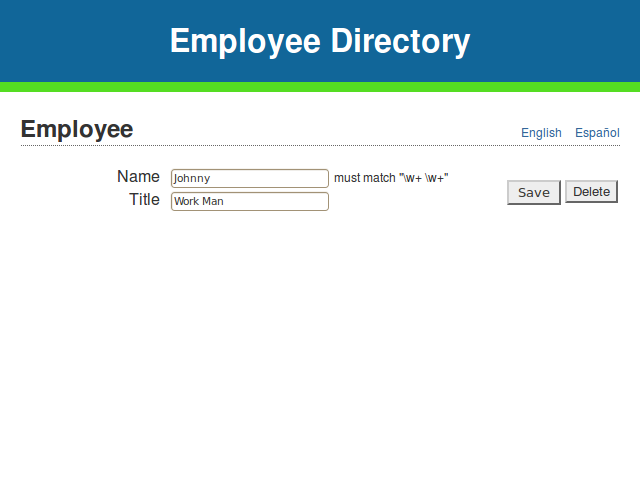
\includegraphics[width=3.2in,height=2.4in]{images/server-side-validation/employee.png}}
\end{center}
\caption{A server-side validation error}
\label{fig:server-side-validation/employee}
\end{figure}

\subsection{Section References}

\begin{itemize}
\item Spring's support for the \texttt{@Valid} annotation is covered in the \href{http://static.springsource.org/spring/docs/3.0.x/spring-framework-reference/html/validation.html#validation-mvc-triggering}{Spring 3 Reference, section 5.7.4.1}.
\item The \texttt{BindingResult} and data binding are covered in the \href{http://static.springsource.org/spring/docs/3.0.x/spring-framework-reference/html/validation.html#validation-binder}{Spring 3 Reference, section 5.7.3}.
\item Spring's support for the JSR-303 Bean Validation API is covered in the \href{http://static.springsource.org/spring/docs/3.0.x/spring-framework-reference/html/validation.html#validation-beanvalidation-overview}{Spring 3 Reference, section 5.7.1}.
\end{itemize}

\pagebreak
\section{Rich Client-Side Validation}

The counterpart to server-side validation is client-side validation, which is made easy by Spring JavaScript.

\subsection{Additions}

The following additions are required:

\begin{itemize}
\item \texttt{spring-js} to the Maven POM
\item The Spring JavaScript \texttt{ResourceServlet} to the Web deployment descriptor
\item Dojo and Spring JavaScript scripts and layout to the views
\item Spring JavaScript validation decorators to the views
\end{itemize}

\subsection{Web Configuration}

Spring JavaScript includes \texttt{ResourceServlet}, which provides various scripts and CSS layouts from both Dojo and Spring JavaScript.  These add the functionality and look-and-feel needed for rich client-side validation.  The \texttt{ResourceServlet} must be added to the Web deployment descriptor.

\lstinputlisting[caption=web.xml,language=xml]{source-code/client-side-validation/web.xml}

\subsection{View Templates}

The Dojo and Spring JavaScript scripts and layout must be added to each view which will provide rich client behavior.

\lstinputlisting[caption=employee.jsp,language=html]{source-code/client-side-validation/employee-head.jsp}

Spring JavaScript uses the decorator pattern to cleanly introduce rich client behavior into views.  Script-free HTML is first built to create a fully functioning application, and Spring JavaScript decorators are added \emph{on top of} the existing DOM to introduce rich behavior.  This means that a view is fully functional on its own, which allows the application to run in an environment where JavaScript support might be limited or non-existent.

This practice, known as progressive enhancement, allows a Web application to remain functional across a wealth of browsers, which may vary in their level of support of JavaScript and CSS.  The most important takeaway from this idea is that the \texttt{onclick} attribute is never directly used in HTML code.  It is only accessed by a decorator, meaning its behavior is only used when the decorator script itself is supported.

The form in \texttt{employee.jsp} is updated to insert Spring JavaScript decorators.

\lstinputlisting[caption=employee.jsp,language=html]{source-code/client-side-validation/employee-body.jsp}

Field decorators have been added to all of the form input fields, and a global validation director has been added to the form submission button.  These are just a few examples of the vast set of features provided by Dojo.

The \emph{employee} form will now validate on the client, displaying any validation errors dynamically.  An example of this is shown in Figure \ref{fig:client-side-validation/employee}.

\vspace{10pt}
\begin{figure}[H]
\begin{center}
\fbox{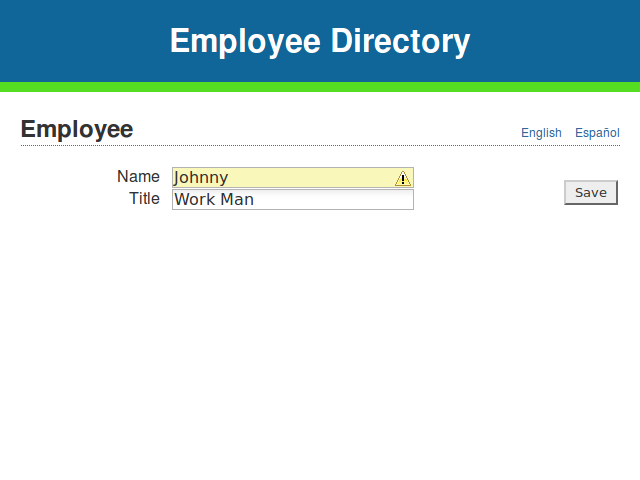
\includegraphics[width=3.2in,height=2.4in]{images/client-side-validation/employee.png}}
\end{center}
\caption{A client-side validation error}
\label{fig:client-side-validation/employee}
\end{figure}

\subsection{Section References}

\begin{itemize}
\item Spring JavaScript is currently part of Spring Web Flow, and documentation is available in the \href{http://static.springsource.org/spring-webflow/docs/2.0.x/reference/html/ch11s04.html}{Spring Web Flow 2 Reference, section 11.4}.
\item Dojo form widgets are documented in detail in Dojo's \href{http://docs.dojocampus.org/dijit/form/}{Dijit documentation}.
\end{itemize}

\pagebreak
\section{Security}

A Web application would seldom be complete without at least a minimal security layer to prohibit unauthenticated access to protected resources.  In this section, basic security is introduced by adding HTML form-based authentication using Spring Security.

\subsection{Additions}

The following additions are required:

\begin{itemize}
\item Spring Security to the Maven POM
\item Spring Security's \texttt{DelegatingFilterProxy} to the Web deployment descriptor
\item An aplication-level Spring context containing Spring Security configuration
\end{itemize}

\subsection{Web Configuration}

Spring Security's \texttt{DelegatingFilterProxy} is essentially a J2EE \texttt{Filter} which nominally handles all requests and determines how to allow or reject access.

\lstinputlisting[caption=web.xml,language=xml]{source-code/security/web.xml}

\subsection{Spring Configuration}

Spring's \texttt{ContextLoaderListener} is needed because there is now a parent Spring context which is extended by the \texttt{spring-mvc} context of before.  The \texttt{contextConfigLocation} parameter specifies the location of the new parent configuration file.

\lstinputlisting[caption=spring-mvc-security.xml,language=xml]{source-code/security/spring-mvc-security.xml}

This nearly minimal configuration sets up an in-memory repository of roles, and enforces access to every resource against this repository.  Here, a form-based login page is provided by Spring, as shown in Figure \ref{fig:security/login-page}.

\vspace{10pt}
\begin{figure}[H]
\begin{center}
\fbox{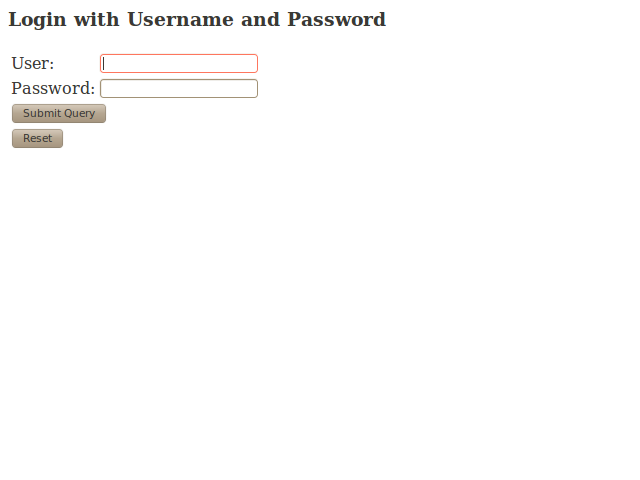
\includegraphics[width=3.2in,height=2.4in]{images/security/login-page.png}}
\end{center}
\caption{Spring Security form-based login page}
\label{fig:security/login-page}
\end{figure}

\subsection{Section References}

\begin{itemize}
\item Java Servlet Filters are covered in \href{http://www.oracle.com/technetwork/java/filters-137243.html}{The Essentials of Filters}, from Oracle.
\item The \href{http://static.springsource.org/spring-security/site/}{Spring Security} Web site contains the reference documentation, plus useful links to literature and examples.
\end{itemize}

\pagebreak
\section{Database Integration}

A major component of enterprise applications is information storage and retrieval via a relational database.  Most of this behavior is confined to a special data tier, with a thin API exposed to the application tier for interaction with the domain.  In this section, a Hibernate-based data tier is introduced for storage and retrieval of data.

\subsection{Additions}

The following additions are required:

\begin{itemize}
\item Multiple libraries to the Maven POM, including \texttt{hibernate}, \texttt{hibernate-annotations}, \texttt{persistence-api}, \texttt{jta}, \texttt{spring-orm}, \texttt{commons-dbcp}, and \texttt{hsqldb}
\item JPA annotations on \texttt{Employee}
\item A repository to provide database interaction
\item Integration of \texttt{EmployeeController} with the repository
\item A new Spring context, \texttt{persistence-context.xml}
\item Optional externalization of the \texttt{DataSource} via JNDI
\end{itemize}

\subsection{Classes}

A persistable type is created to represent the domain model.  In this simple example, this will closely resemble the UI model, but it is important to draw a distinction between the two, as they serve two very different purposes.

The purpose of a domain model is to represent the domain model.  The purpose of a UI model is to represent the UI model.  This is intentionally redundant, because it is easy to forget.  The domain model can include potentially complex object hierarchies as well as database-specific metadata.  The UI model will have forms and other data structures which will tend to be very flat, and contain very specific information meant to be rendered in a view.

Attempting to merge the two models can get painfully cumbersome, as the domain model tends not to map directly to the UI model.  Furthermore, the resulting tight coupling will force any changes in one to necessitate changes in the other.  It is much simpler to create simple conversion logic in the service tier to translate between the two models.

The \texttt{Employee} class is made persistable with JPA annotations.

\lstinputlisting[caption=Employee.java]{source-code/database/Employee.java}

A repository serves the domain as an opaque entry point into the database.  It provides accessors and mutators for database tables represented only by domain objects.

\lstinputlisting[caption=HibernateEmployeeService.java]{source-code/database/HibernateEmployeeService.java}

This repository is meant to work with Hibernate, and so uses a Hibernate \texttt{SessionFactory}.

In this example, the service tier is contained entirely within \texttt{EmployeeController}, which is modified to interact with the new repository.

\texttt{BindableEmployee} provides an \texttt{Employee}-based constructor plus two helper methods, \texttt{asEmployee()} and \texttt{bindableEmployee(Collection<Employee>)}, which do the mapping between the UI model and the domain model.

\lstinputlisting[caption=BindableEmployee.java]{source-code/database/BindableEmployee.java}

\subsection{Spring Configuration}

Next, a new global Spring context is created to manage the database-related objects.

\lstinputlisting[caption=persistence-context.xml,language=xml]{source-code/database/persistence-context.xml}

This context is made a parent context via \texttt{ContextLoaderListener} in the Web deployment descriptor.

\lstinputlisting[caption=web.xml,language=xml]{source-code/database/web.xml}

A minor change is required in \texttt{spring-mvc-servlet.xml} to enable service tier transaction management.

\lstinputlisting[caption=spring-mvc-servlet.xml,language=xml]{source-code/database/spring-mvc-servlet.xml}

The \texttt{DataSource} can optionally be externalized from the Spring configuration via JNDI.  Configuration specifics, such as database username and password, are then kept out of the Spring configuration and delegated to the application server.  This adds security by allowing the application server protect these sensitive data.  For Apache Tomcat, the \texttt{DataSource} is added to \texttt{META-INF/context.xml}.

\lstinputlisting[caption=context.xml,language=xml]{source-code/database/context.xml}

The \texttt{DataSource} bean is removed from the Spring configuration, and replaced by a JNDI-lookup:

\lstinputlisting[caption=persistence-context.xml,language=xml]{source-code/database/persistence-context-jndi.xml}

\subsection{Section References}

\begin{itemize}
\item JPA annotations are part of the Java Persistence API, which is covered in \href{http://en.wikipedia.org/wiki/Java_Persistence_API}{Wikipedia}.
\item Spring's \texttt{jee} namespace provides easy JNDI integration, and is covered in the \href{http://static.springsource.org/spring/docs/3.0.x/spring-framework-reference/html/xsd-config.html#xsd-config-body-schemas-jee}{Spring Reference, section C.2.3}.
\item Hibernate documentation is available from \href{http://docs.jboss.org/hibernate/stable/core/reference/en/html/}{JBoss}.
\item The multi-tier architecture is covered in \href{http://en.wikipedia.org/wiki/Multitier_architecture}{Wikipedia}.
\end{itemize}

\pagebreak
\section{RESTful Web Services}

One of the awesome features of the Spring MVC is its ability to easily support multiple types of request/response content.  In fact, the same Spring MVC beans can be used to serve conventional HTML, RESTful XML, JSON, Atom, etc. usually with only some minor configuration changes.

This section introduces a RESTful Web service which utilizes the existing Spring MVC beans and configuration.

\subsection{Additions}

The following additions are required:

\begin{itemize}
\item JAXB annotations to \texttt{BindableEmployee} to define its XML marshalling configuration
\item The \texttt{spring-oxm} library to the Maven POM
\item A supplement to the \texttt{InternalResourceViewResolver} in the Spring context with a \texttt{ContentNegotiatingViewResolver} and some JAXB marshalling configuration
\end{itemize}

\subsection{Classes}

JAXB annotations are similar in use to Hibernate annotations.  In this example, \texttt{BindableEmployee} is simple and flat enough that it will marshal easily with a few JAXB annotations.

\lstinputlisting[caption=BindableEmployee.java]{source-code/rest/BindableEmployee.java}

Spring MVC needs the ability to choose an appropriate view resolver depending on the specifics of the request.  When a conventional \texttt{text/html} request is made from a Web browser, Spring MVC uses an \texttt{InternalResourceViewResolver} to delegate to a JSP view template as before.  When an \texttt{application/xml} request is made by a Web service consumer, Spring MVC uses a \texttt{MarshallingView} with a JAXB marshaller to provide an XML representation of the \texttt{BindableEmployee}.

\subsection{Spring Configuration}

\lstinputlisting[caption=spring-mvc-servlet.xml,language=xml]{source-code/rest/spring-mvc-servlet.xml}

\subsection{Testing}

The HTML/XML duality of this example can be tested with \texttt{curl}:

\begin{lstlisting}[language=bash]
> curl -H 'Accept: application/xml' localhost:8080/barebones-spring-mvc/employee
> curl -H 'Accept: text/html' localhost:8080/barebones-spring-mvc/employee
\end{lstlisting}

\subsection{Section References}

\begin{itemize}
\item Java Architecture for XML Binding (JAXB) is covered by \href{http://www.oracle.com/technetwork/articles/javase/index-140168.html}{Oracle}.
\item Representational State Transfer (REST) is covered in \href{http://en.wikipedia.org/wiki/Representational_State_Transfer}{Wikipedia}
\item Spring's comprehensive REST support is covered in the \href{http://static.springsource.org/spring/docs/3.0.x/spring-framework-reference/html/new-in-3.html#d0e1188}{Spring 3 Reference}
\item cURL is covered by the \href{http://curl.haxx.se/docs/manual.html}{cURL manual}.
\end{itemize}

\pagebreak
\section{Externalization and Internationalization}

Message externalization in the Web view layer digs the various text out of view templates and keeps it centralized and manageable.  It also provides a convenient launchpad for site internationalization.  Spring MVC provides for easy introduction of message externalization and internationalization into the view layer.

\subsection{Additions}

The following additions are required:

\begin{itemize}
\item A \texttt{ResourceBundleMessageSource} bean to the Spring context
\item A resource bundle, messages.properties, to contain messages from the JSP
\item Message tanslations from \texttt{messages.properties} into Spanish in \texttt{messages\_es.properties}
\item \texttt{LocaleChangeInterceptor} and \texttt{SessionLocaleResolver} beans to the Spring context
\end{itemize}

\subsection{Spring Configuration}

Spring needs to know where it will find externalized messages.  This is done with Java's resource bundle functionality, encapsulated in a Spring \texttt{ResourceBundleMessageSource}.

\lstinputlisting[caption=spring-mvc-servlet.xml,language=xml]{source-code/i18n/spring-mvc-servlet-message-source.xml}

There isn't much in the way of messages in this example, but the little that is there is moved into a properties file named in the above \texttt{ResourceBundleMessageSource}.

\lstinputlisting[caption=message.properties]{source-code/i18n/messages.properties}

This is also done in Spanish.  Translations were performed with the help of \href{http://translate.google.com/}{Google Translate}, so as far as I know nothing below says ``Your mother was a hamster."

\lstinputlisting[caption=messages\_es.properties]{source-code/i18n/messages_es.properties}

Next, a couple of beans are added to the Spring context to allow detection of a user's desire to switch languages, and the ability to store that preference in the user's session.

\lstinputlisting[caption=spring-mvc-servlet.xml,language=xml]{source-code/i18n/spring-mvc-servlet-locale.xml}

A user simply includes the HTTP request parameter \texttt{lang=es} to change the language to Spanish.

\vspace{10pt}
\begin{figure}[H]
\begin{center}
\fbox{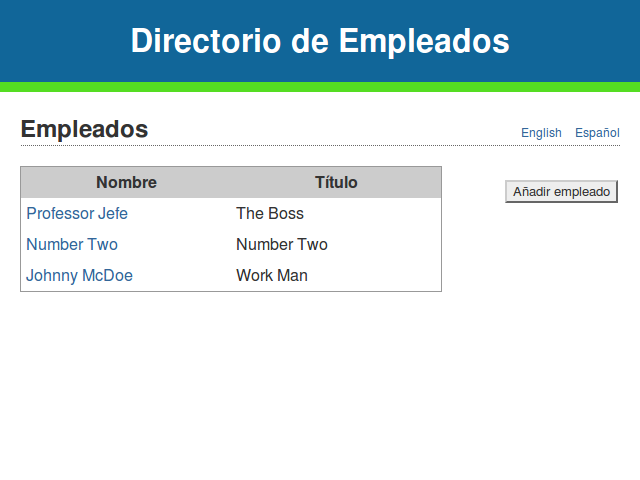
\includegraphics[width=3.2in,height=2.4in]{images/i18n/view-employees-spanish.png}}
\end{center}
\caption{The \emph{employee} view in Spanish}
\label{fig:i18n/view-employees-spanish}
\end{figure}

\pagebreak
\section{References}

\bf{Dijit}

\href{http://docs.dojocampus.org/dijit/form/}{http://docs.dojocampus.org/dijit/form/}

\href{http://www.dojotoolkit.org/reference-guide/dijit/index.html}{http://www.dojotoolkit.org/reference-guide/dijit/index.html}

\bf{Spring 3 Reference}

\href{http://static.springsource.org/spring/docs/3.0.x/spring-framework-reference/html/}{http://static.springsource.org/spring/docs/3.0.x/spring-framework-reference/html/}

\bf{Spring API}

\href{http://static.springsource.org/spring/docs/3.0.x/javadoc-api/}{http://static.springsource.org/spring/docs/3.0.x/javadoc-api/}

\bf{Spring Security}

\href{http://static.springsource.org/spring-security/site/}{http://static.springsource.org/spring-security/site/}

\bf{Spring Web Flow}

\href{http://static.springsource.org/spring-webflow/docs/2.0.x/reference/html/}{http://static.springsource.org/spring-webflow/docs/2.0.x/reference/html/}

\end{document}
